\section*{Example}
Player 2 (top) took the \PPING{} action on their turn.
Because the action name is written is yellow, they played their action card face up.

\vspace{-1ex}

\begin{center}
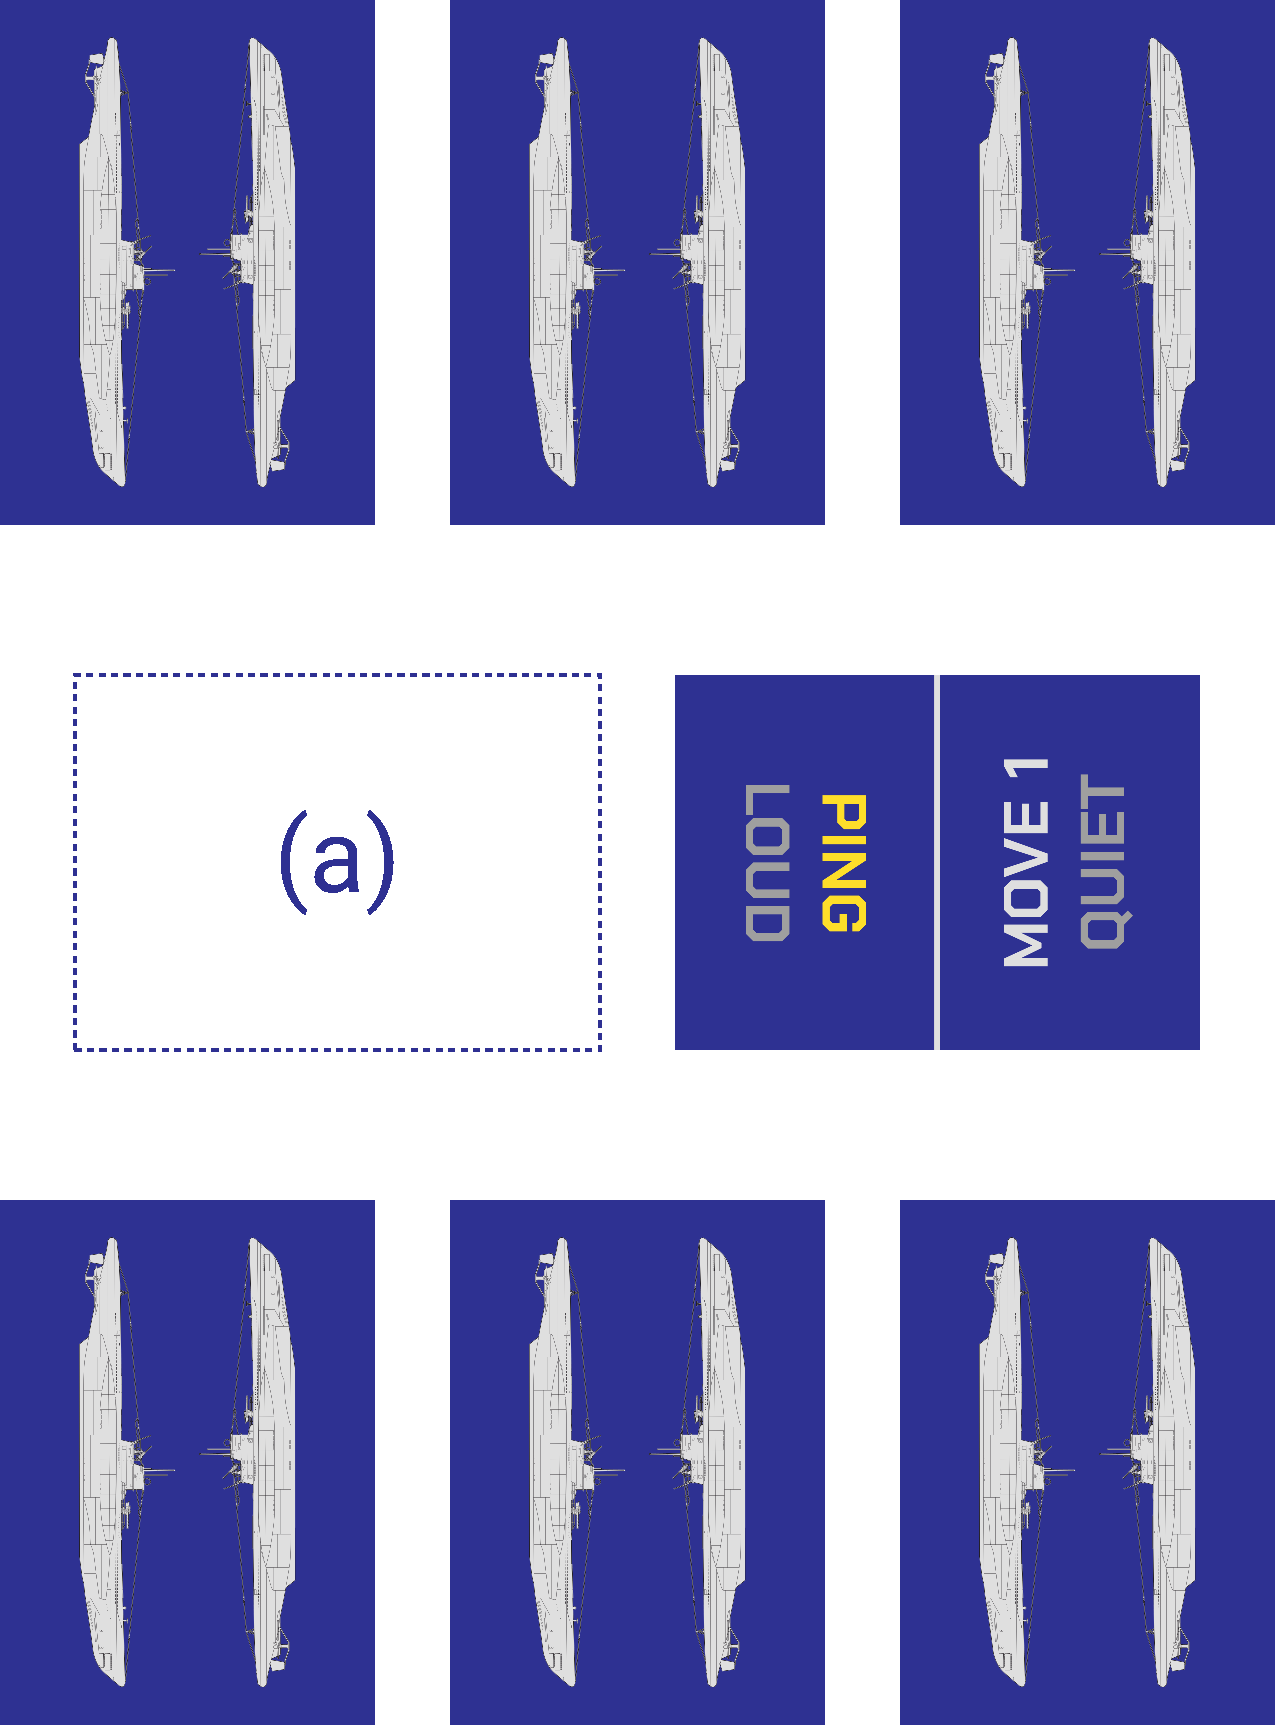
\includegraphics[width=0.5\linewidth]{example_diagram.pdf}
\end{center}

\vspace{-1ex}

Next, Player 1 (bottom) will take an action. They will place the corresponding action card in the play area (a).
Then, they will add the card on the right-hand side of the play area to their hand.
